\chapter{Introduction to limits}
The concept of a limit is extremely fundamental to the understanding of calculus, namely differentiation
and integration; their formal definitions are in terms of limits. Here, we will introduce limits for
sequences and functions, their arithmetic operations, the squeeze theorem, L'Hopital's rule, and
apply it to formally defining the derivative.

One other key use of limits is in evaluating \textit{improper integrals}. For example, one can
evaluate

\[\int_{1}^{\infty} \frac{1}{x^2} \, dx = \lim_{\Omega \to \infty} \int_{1}^{\Omega} \frac{1}{x^2} \, dx = 1\]

The reason we need a limit in this case is because we simply cannot directly evaluate
\[\frac{1}{\infty}\]
Dividing by infinity is not defined in the real numbers! In fact, $\infty \notin \mathbb{\mathbb{R}}$.

\section{Limits of sequences and functions}

\subsection{Limits of sequences}
Suppose we have a sequence
\[
a_1,a_2,a_3,a_4,...
\]
If the term $a_n$ converges to a fixed value $L$ as $n$ tends to infinity, then we write
\[
\lim_{n \to \infty} a_n = L
\]
This is read as ``the \textit{limit} of the sequence ${a_n}$ as $n$ tends to infinity is $L$''.

This concept of a limit can be stated with the following definition:
\begin{definition}
    If, for any arbitrarily small positive number $\epsilon$, one can always find a term in a sequence ${a_n}$
    such that $|a_n - L| < \epsilon$ if $n > N(\epsilon)$, and $N(\epsilon)$ is a function of $\epsilon$.
\end{definition}

A more advanced treatment of limits, and how the above definition can prove common limits, can be found in
\cite{Gong_2017}.

Take note that there are sequences which diverge (i.e. they do not converge). Consider the harmonic series,
where the $n$-th term is \[H_n = \sum_{k = 1}^n \frac{1}{k}\] Although it increases slowly, it can be proven
that \[\lim_{n \to \infty} H_n = \infty\] This proof is left as an exercise to the reader.

\subsection{Limits of functions}
Similar to the above interpretation of limits to sequences, suppose that we have a function
$f(x)$. If $f(x)$ approaches $L$ as $x$ tends to $c$ from both sides (i.e., from $-\infty$, and from $\infty$),
then $\lim_{x \to c} f(x) = L$.

\begin{example}
    Find the limit $\lim_{x \to \infty} \frac{1}{x}$.
\end{example}
\begin{solution}
    The limit is \[\lim_{x \to \infty} \frac{1}{x} = 0.\]
\end{solution}

\section{Approximating limits}
The above sections now beg the question, ``how do we find what a limit is?'' In this section, we will discover the
idea of a `limit', how we can approximate it, and then how we can find the exact value of the limit.

Some functions may not be defined at some particular value, for example
$f(x) = \frac{\sin(x)}{x}$ is not defined at $x = 0$ due to division by zero being undefined.
Instead of leaving it undefined, we can attempt to `complete' the graph of $y = f(x)$, by trying
to find some suitable value; this is where limits come in.

The process of `completing' the graph of $y = f(x)$ at $x = c$ (where $f(c)$ does not exist) will
definitely involve studying the \textit{behavior} of the function around $x = c$. Even if $f(c)$ existed,
we ignore that, and find our own `completion' to the graph.

We will start with this idea of `completing the graph' in the following section, using numerical methods first.

Consider the function $f(x) = \frac{\sin(x)}{x}$, where $x$ is in degrees. If we graph it, we get:

\begin{figure}[h]
    \centering
    \begin{tikzpicture}
        \begin{axis}[
            axis lines = middle,
            xlabel = $x$,
            ylabel = {$y$},
            domain=-10:10,
            samples=200,
            ymin=-0.5, ymax=1.5,
            restrict y to domain=-2:2,
            ]
            \addplot[
                domain=-10:-0.1,
                samples=100,
                thick,
                smooth,
            ]{sin(deg(x))/x};
            \addplot[
                domain=0.1:10,
                samples=100,
                thick,
                smooth,
            ]{sin(deg(x))/x};
            \addplot[
                only marks,
                mark=*,
                mark options={fill=white, draw=black},
            ] coordinates {(0, 1)};
        \end{axis}
    \end{tikzpicture}
    \caption{Plot of $y = \frac{\sin(x)}{x}$}
    \label{fig:sincx}
\end{figure}

In Figure \ref{fig:sincx}, $y$ is not defined at $x = 0$ since division by zero is undefined. However, $y$ can be seen
approaching $1$ as $x \to 0$, \textbf{from both sides}. In limit notation, $\lim_{x \to 0} y = 1$.

(One-sided limits, where $x$ approaches from only one side, will be covered later.)

Now, let us define a sequence where the $n$-th term
\[T_n = \frac{\sin(n)}{n}\]
for $n \in \mathbb{Z}^+$.

\begin{table}
    \centering
    \begin{tblr}{cells = {c}, hlines, vlines}
        $-\lg(n)$ & $T_n$ (approx.)  \\
        $1$ & $0.99833416647$  \\
        $2$ & $0.999983333417$ \\
        $3$ & $0.99999983333$  \\
        $4$ & $0.99999999833$  \\
        $5$ & $0.99999999983$  
    \end{tblr}
    \caption{Values of $-\lg(n)$ and $T_n$ for $0 \le n \le 5$.}
    \label{tab:vntn}
\end{table}

As seen in Table \ref{tab:vntn}, $T_n$ quickly approaches $1$ as $n$ approaches zero. In notation,
\[T_n \to 1\,\,\text{as}\,\,n \to 0\]
In other words,
\[\lim_{n \to 0} T_n = \lim_{n \to 0} \frac{\sin(n)}{n} = 1\]

The reason that we can find the limit like so, is because $\frac{\sin(x)}{x}$ actually approaches
\textbf{only one} value (from both sides), as seen in Figure \ref{fig:sincx}.

Contrast this with the function $f(x) = \sin\left(\frac{1}{x}\right)$.

\begin{figure}
    \centering
    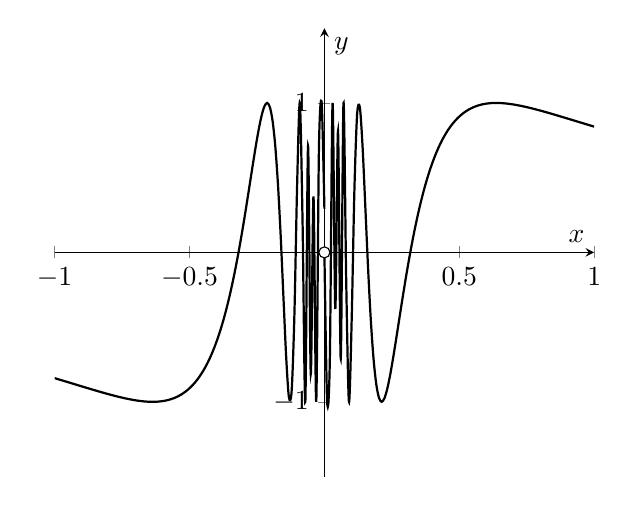
\begin{tikzpicture}
        \begin{axis}[
            axis lines = middle,
            xlabel = $x$,
            ylabel = {$y$},
            domain=-1:1,
            samples=200,
            ymin=-1.5, ymax=1.5,
            restrict y to domain=-2:2,
            ]
            \addplot[
                domain=-1:-0.00001,
                samples=100,
                thick,
                smooth,
            ]{sin(deg(1/x))};
            \addplot[
                domain=0.00001:1,
                samples=100,
                thick,
                smooth,
            ]{sin(deg(1/x))};
            \addplot[
                only marks,
                mark=*,
                mark options={fill=white, draw=black},
            ] coordinates {(0, 0)};
        \end{axis}
    \end{tikzpicture}
    \caption{Plot of $y = f(x) = \sin\left(\frac{1}{x}\right)$}
    \label{fig:sinrx}
\end{figure}

As seen in Figure \ref{fig:sinrx}, $y = f(x)$ oscillates wildly. It does not even approach a value as $f(x)$ gets smaller; we will leave
the verification of this to the reader. Hence, the limit does not exist here, as $f(x)$ never converges to any
particular value.

In fact, the limit does not even need to exist. Consider the sign function $\sgn(x)$, where
$\sgn(x) = -1$ for $x < 0$, $\sgn(x) = 1$ for $x > 0$ and $\sgn(x) = 0$ for $x = 0$, and its
graph in Figure \ref{fig:sgn}.

We know that $\sgn(x)$ is defined everywhere, including $0$. However, limits study the behavior of
functions \textit{around} some point, not \textit{at} that point.

If we look from the left of Figure \ref{fig:sgn}, it seems like $\sgn(x)$ is approaching $-1$ as $x$ approaches $0$ from
$-\infty$. However, from the right, it seems like $\sgn(x)$ is approaching $1$ as $x$ approaches $0$
from $+\infty$ (the positive sign is explicitly used here to emphasize that we approach from the right).

Hence, because $\sgn(x)$ does not settle on only one value when $x$ approaches $0$ from both sides
(i.e., the values are different, as stated previously), the limit of $\sgn(x)$ as $x \to 0$ \textbf{does
not exist}.

Note that $\lim_{x \to 0} \sgn(x) \ne \sgn(0)$. Compare this with any polynomial; all polynomials $P(x)$
satisfy the property \[\forall (P : \mathbb{R} \to \mathbb{R}) \forall c \in \mathbb{R} \to \mathbb{R} : \lim_{x \to c} P(x) = P(c)\]
This property is very important; it is called \textit{continuity}. It will be discussed later.

\begin{figure}
    \centering
    \begin{tikzpicture}
        \begin{axis}[
            axis lines = middle,
            xlabel = $x$,
            ylabel = {$y$},
            domain=-1:1,
            samples=200,
            ymin=-1.5, ymax=1.5,
            restrict y to domain=-2:2,
            ]
            \addplot[
                domain=-1:-0.00001,
                samples=100,
                thick,
                smooth,
            ]{-1};
            \addplot[
                domain=0.00001:1,
                samples=100,
                thick,
                smooth,
            ]{1};
            \addplot[
                only marks,
                mark=*,
                mark options={fill=black, draw=black},
            ] coordinates {(0, 0)};
        \end{axis}
    \end{tikzpicture}
    \caption{Plot of $y = \sgn(x)$}
    \label{fig:sgn}
\end{figure}

\newpage

\section{Basic laws of limits}
Before we prepare for evaluating limits' exact values, we must make ourselves aware of the following laws.
We distinguish this section from the following, so the reader can easily reference this section.

Suppose that $\lim_{x \to c} f(x) = A$ and $\lim_{x \to c} g(x) = B$ for the functions $f(x)$, $g(x)$,
and $A,B$ are constants. Then:

\begin{itemize}
    \item \textbf{Sum and Difference Law}
    \[
    \lim_{x \to c} (f(x) \pm g(x)) = A \pm B,
    \]
    \item \textbf{Product Law}
    \[
    \lim_{x \to c} (f(x) g(x)) = A B,
    \]
    \item \textbf{Quotient Law}
    \[
    \lim_{x \to c} \left(\frac{f(x)}{g(x)}\right)  = \frac{A}{B},\,\,B\ne 0,
    \]
    \item \textbf{Constant Multiple Law}
    \[
    \lim_{x \to c} kf(x) = k\lim_{x \to c} f(x) = kA,\,\,k\,\,\text{is a constant}
    \]
    \item \textbf{Power Law}
    \[
    \lim_{x \to c} (f(x))^k = (\lim_{x \to c} f(x))^k = A^k,\,\,k \in \mathbb{Z^+}
    \]
    \item \textbf{Root Law for (for $A < 0$)}
    \[
    \lim_{x \to c} \sqrt[k]{f(x)} = \sqrt[k]{\lim_{x \to c} f(x)} = \sqrt[k]{A},\,\,A < 0, k \in \mathbb{Z^+}
    \setminus \{2, 4, 6, 8, ...\}
    \]
    \item \textbf{Root Law (for all other cases)}
    \[
    \lim_{x \to c} \sqrt[k]{f(x)} = \sqrt[k]{\lim_{x \to c} f(x)} = \sqrt[k]{A},\,\,A \ge 0, k \in \mathbb{Z^+}
    \]
    \item \textbf{Basic Law 1}
    \[
    \lim_{x \to c} x = c
    \]
    \item \textbf{Basic Law 2}
    \[
    \lim_{x \to c} k = k, \quad \text{$k$ is a constant}
    \]
\end{itemize}

(In examinations, do not state ``Basic Law 1'' and ``Basic Law 2''! They are just names given for
easy reference in this book.)

\begin{example}
    Find the limit of \[\frac{k}{e^x} + \frac{1}{x^2}\] as $x$ tends to some unknown $c \in \mathbb{R}$
    (in other words, $c$ is finite),
    in terms of $A$ and $B$ where \[\lim_{x \to c} e^x = A, \lim_{x \to c} x^2 = B.\]
    State the laws applied.
\end{example}
\begin{solution}
    \begin{equation*}
        \begin{split}
            \lim_{x \to c} \left(\frac{k}{e^x} + \frac{1}{x^2}\right)
            &= \lim_{x \to c} \frac{k}{e^x} + \lim_{x \to c} \frac{1}{x^2} \quad \text{(Sum Law)} \\
            &= \frac{\lim_{x \to c} k}{\lim_{x \to c} e^x} + \frac{\lim_{x \to c} 1}{\lim_{x \to c} x^2} \quad
            \text{(Quotient Law)} \\
            &= \frac{k}{\lim_{x \to c} e^x} + \frac{1}{\lim_{x \to c} x^2} \quad
            \text{(Basic Law 2)} \\
            &= \frac{k}{A} + \frac{1}{B} \quad
            \text{(by definition of $A$ and $B$)} \\
        \end{split}
    \end{equation*}
\end{solution}

\section{Algebraic evaluation of limits}
Let us start off this section by recognizing that there are inherent problems with graphs.
While graphs are great for studying functions, they provide limited precision for approximating
limits; in the interest of accuracy, we usually pick algebraic methods of evaluation compared to approximation.

In order to evaluate a limit algebraically, we must be able to transform it such that we can directly substitute
in values without any problems like dividing by infinity.

\section{The squeeze theorem}
The squeeze theorem is extremely useful in determining important limits; in fact, it is key to proving the
derivative of $\sin(x)$ (with respect to $x$). Hence, we begin with a statement of the theorem.

\begin{theorem}[Squeeze theorem]\thlabel{squeeze}
    Suppose that we have three functions $f(x), g(x), h(x)$ such that $g(x)\le f(x)\le h(x)$. Then
    \[
    \lim_{x \to c} g(x) = \lim_{x \to c} h(x) = L \implies \lim_{x \to c} f(x) = L
    \]
    where $c$ is a constant.
\end{theorem}
\begin{proof}
    The proof is beyond the scope of this book.
\end{proof}

Now, we begin with some examples.

\begin{example}
    Find the limit \[\lim_{x \to 0}x^2\sin\left(\frac{1}{x}\right).\]
\end{example}
\begin{solution}
    We cannot apply the law
    \[
    \lim_{x \to c} (f(x) g(x)) = A B
    \]
    because $\lim_{x \to 0} \sin\left(\frac{1}{x}\right)$ does not exist. However, since the range of $\sin(x)$
    is $[-1, 1]$, we can establish the inequality \[-1 \le \sin\left(\frac{1}{x}\right) \le 1.\] Multiplying both
    sides by $x^2$, we obtain \[-x^2 \le x^2 \sin\left(\frac{1}{x}\right) \le x^2.\]
    Evaluating the leftmost and
    rightmost limits by direct substitution,
    \[\lim_{x \to 0} x^2 = \lim_{x \to 0} (-x^2) = 0 \implies
    \lim_{x \to 0} x^2 \sin\left(\frac{1}{x}\right) = 0 \]
    by the squeeze theorem, and we are done.
\end{solution}

\section{Differentiation from first principles}
Differentiation in the `A'-Level and `O'-Level has, in the author's experience, only been taught in terms of
memorizing formulae and identities. For example, one simply assumes that \[\frac{d}{dx}\sin(x) = \cos(x).\]

The proof of this `trivial' identity, is not `trivial'; it has never ever been covered in any
ordinary course. This is because the proof of this identity utilizes \thref{squeeze}.
In fact, most trigonometric identities stem from the aforementioned theorem.

Now, we must start with the very definition of what a
derivative is. Instead of introducing the definition directly without further explanation, let us
briefly derive the definition of the derivative ourselves.

Recall that the gradient of a straight line $y$ passing through two points $(x_1, y_1)$ and $(x_2, y_2)$ is
defined as $m = \frac{y_2 - y_1}{x_2 - x_1}.$, where $x_2 > x_1$ and $x,y \in \mathbb{R}$.
If $y = f(x)$, then $m = \frac{f(x_2) - f(x_1)}{x_2 - x_1}.$ If this straight line passes through some curve,
and the line is \textbf{not} a tangent to that curve (i.e., it intersects the curve more than once),
the straight line is known as a \textit{secant line} of that curve.

\begin{figure}
    \centering
    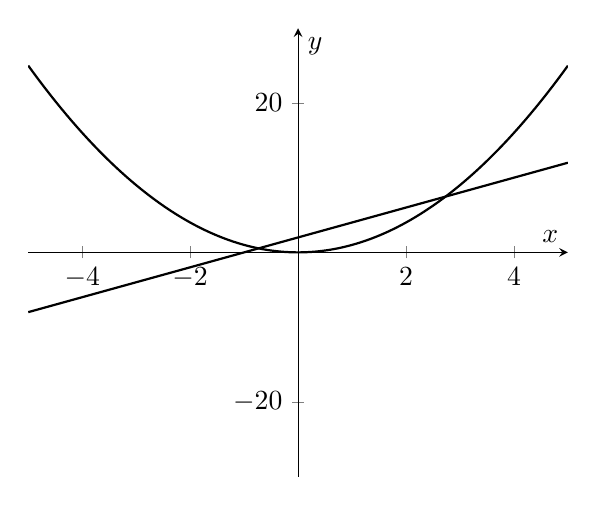
\begin{tikzpicture}
        \begin{axis}[
            axis lines = middle,
            xlabel = $x$,
            ylabel = {$y$},
            domain=-5:5,
            samples=200,
            ymin=-30, ymax=30,
            restrict y to domain=-30:30,
            ]
            \addplot[
                domain=-5:5,
                samples=100,
                thick,
                smooth,
            ]{x^2};
            \addplot[
                domain=-5:5,
                samples=100,
                thick,
                smooth,
            ]{2*x+2};
        \end{axis}
    \end{tikzpicture}
    \caption{
        Plot of $y = x^2$ and one of its secant lines $y = 2x + 2$.
        Notice that as the distance between the points which the secant line intersects get closer
        to a single point, we get a better approximation of the tangent of the curve at that point.
    }
    \label{fig:secantline}
\end{figure}

Now, consider the difference between $x_2$ and $x_1$; let this difference be
$\delta = x_2 - x_1$. Then $x_2 = x_1 + \delta$. Replacing all such occurences of $x_2$, one obtains
\[m = \frac{f(x_1 + \delta) - f(x_1)}{\delta}.\]

We have learnt that we can draw a tangent at a point in a graph to find the gradient at that point; this is exactly
the idea we use here to formally define the derivative. As $\delta$ tends to $0$, we will get a better approximation
of the gradient at the point $(x_1, y_1)$. Alas, using limits, we have the following definition:

\begin{definition}
    The derivative of a function $f(x)$, with respect to $x$, is defined as
    \[f'(x) = \lim_{\delta \to 0} \frac{f(x + \delta) - f(x)}{\delta}\]
\end{definition}

When we apply this definition in finding a derivative, the process is dubbed as \textit{differentiating
from first principles}.

\begin{example}
    Find the derivative of $f(x) = 3x^2 + 2x + 1$.
\end{example}
\begin{solution}
    By differentiating from first principles, one obtains
    \begin{equation*}
        \begin{split}
            f'(x) &= \lim_{\delta \to 0} \frac{f(x + \delta) - f(x)}{\delta} \\
            &= \lim_{\delta \to 0} \frac{(3(x + \delta)^2 + 2(x + \delta) + 1) - (3x^2 + 2x + 1)}{\delta} \\
            &= \lim_{\delta \to 0} \frac{3(x + \delta)^2 + 2x + 2\delta + 1 - 3x^2 - 2x - 1}{\delta} \\
            &= \lim_{\delta \to 0} \frac{3(x + \delta)^2 + 2\delta - 3x^2}{\delta} \\
            &= \lim_{\delta \to 0} \frac{3(x^2 + 2x\delta + \delta^2) + 2\delta - 3x^2}{\delta} \\
            &= \lim_{\delta \to 0} \frac{3x^2 + 6x\delta + 3\delta^2 + 2\delta - 3x^2}{\delta} \\
            &= \lim_{\delta \to 0} \frac{6x\delta + 3\delta^2 + 2\delta}{\delta} \\
            &= \lim_{\delta \to 0} 6x + 3\delta + 2 \\
            &= 6x + 3(0) + 2 \\
            &= 6x + 2
        \end{split}
    \end{equation*}
    Indeed, this is what we expect since \[\frac{d}{dx}(3x^2 + 2x + 1) = 6x + 2.\]
    Hence we are done.
\end{solution}

\section{L'H\^{o}pital's rule}
L'H\^{o}pital's rule is a theorem popularly used to evaluate limits of expressions which take,
after direct substitution, $\frac{f(x)}{g(x)} = \frac{0}{0}$ or $\frac{\infty}{\infty}$.
If we assume that $f(x)$ and $g(x)$ are differentiable everywhere, and they are well defined
everywhere, we state L'H\^{o}pitals rule as follows:

\begin{theorem}[L'H\^{o}pital's rule]
    For any functions $f : \mathbb{R} \to \mathbb{R}$ and $g : \mathbb{R} \to \mathbb{R}$ differentiable everywhere and well-defined
    everywhere,
    \[\lim_{x \to c} \frac{f(x)}{g(x)} = \lim_{x \to c} \frac{f'(x)}{g'(x)}\]
    if the following conditions hold:
    \begin{itemize}
        \item $\lim_{x \to c} f(x) = \lim_{x \to c} g(x) = 0 \,\,\text{or}\,\pm \infty$
        \item $g'(x) \ne 0$
        \item $\lim_{x \to c} \frac{f'(x)}{g'(x)}$ exists
    \end{itemize}
    where $f(x),g(x)$ are functions of $x$.
\end{theorem}

\newpage
\section{Exercises}

\begin{exercise}
    approximate the limit of $\frac{1}{x}$ as $x$ approaches $0$ from both sides
    (i.e., approximate the left and right limits). Hence, explain why
    \[\lim_{x \to 0} \frac{1}{x}\]
    does not exist.
\end{exercise}

\begin{exercise}
    Prove that \[\lim_{x \to 0} |f(x)| = 0 \implies \lim_{x \to 0} f(x) = 0\]
    using the squeeze theorem. (Hint: $|-f(x)| = |f(x)|$. Form an inequality.)
\end{exercise}

\begin{exercise}
    It is known that the sum of a geometric series up to $n$ terms is given by
    \[S_n = \sum_{k=1}^n ar^{k - 1} = \frac{a(r^n - 1)}{r - 1}\]
    If $|r| < 0$, take the limit of $S_n$ as $n$ approaches $\infty$.
\end{exercise}